%%%%%%%%%%%%%%%%%%%%%%%%%%%%%%%%%%%%%%%%%%
%                                        %
% Szablon pracy dyplomowej magisterskiej % 
%                                        %
%%%%%%%%%%%%%%%%%%%%%%%%%%%%%%%%%%%%%%%%%%



\documentclass[a4paper,twoside,12pt]{book}
\usepackage[utf8]{inputenc}
\usepackage[T1]{fontenc}
\usepackage{amsmath,amsfonts,amssymb,amsthm}
\usepackage[british,polish]{babel}
\usepackage{indentfirst}
\usepackage{lmodern}
\usepackage{graphicx}
\usepackage{hyperref}
\usepackage{booktabs}
\usepackage{tikz}
\usepackage{pgfplots}
\usepackage{mathtools}
\usepackage[page]{appendix} % toc,
\renewcommand{\appendixtocname}{Dodatki}
\renewcommand{\appendixpagename}{Dodatki}
\renewcommand{\appendixname}{Dodatek}

\usepackage{setspace}
\onehalfspacing


\frenchspacing

\usepackage{listings}
\lstset{
language={},
basicstyle=\ttfamily,
keywordstyle=\lst@ifdisplaystyle\color{blue}\fi,
commentstyle=\color{gray}
}

%%%%%%%%%

%%%% LIST GENERATOR %%%%%%%%%

%\usepackage{tikz}
%\usepackage{manfnt}   % dangerous sign 
\usepackage{color}
\definecolor{brickred}      {cmyk}{0 , 0.89, 0.94, 0.28}

\makeatletter \newcommand \kslistofremarks{\section*{Uwagi} \@starttoc{rks}}
\newcommand\l@uwagas[2]
{\par\noindent \textbf{#2:} %\parbox{10cm}
{#1}\par} \makeatother


\newcommand{\ksremark}[1]{%
{%\marginpar{\textdbend}
{\color{brickred}{[#1]}}}%
\addcontentsline{rks}{uwagas}{\protect{#1}}%
}

\newcommand{\comma}{\ksremark{przecinek}}
\newcommand{\nocomma}{\ksremark{bez przecinka}}
\newcommand{\styl}{\ksremark{styl}}
\newcommand{\ortografia}{\ksremark{ortografia}}
\newcommand{\fleksja}{\ksremark{fleksja}}
\newcommand{\pauza}{\ksremark{pauza `--', nie dywiz `-'}}
\newcommand{\kolokwializm}{\ksremark{kolokwializm}}

%%%%%%%%%%%%%% END OF GENERATOR %%%%%%%%%%%

%%%%%%%%%%%% ZYWA PAGINA %%%%%%%%%%%%%%%
% brak kapitalizacji zywej paginy
\usepackage{fancyhdr}
\pagestyle{fancy}
\fancyhf{}
\fancyhead[LO]{\nouppercase{\it\rightmark}}
\fancyhead[RE]{\nouppercase{\it\leftmark}}
\fancyhead[LE,RO]{\it\thepage}


\fancypagestyle{tylkoNumeryStron}{%
\fancyhf{}
\fancyhead[LE,RO]{\it\thepage}
}

\fancypagestyle{NumeryStronNazwyRozdzialow}{%
\fancyhf{}
\fancyhead[LO]{\nouppercase{\it\rightmark}}
\fancyhead[RE]{\nouppercase{\it\leftmark}}
\fancyhead[LE,RO]{\it\thepage}
}


%%%%%%%%%%%%% OBCE WTRETY  
\newcommand{\obcy}[1]{\emph{#1}}
\newcommand{\ang}[1]{{\selectlanguage{british}\obcy{#1}}}
%%%%%%%%%%%%%%%%%%%%%%%%%%%%%

% polskie oznaczenia funkcji matematycznych
\renewcommand{\tan}{\operatorname {tg}}
\renewcommand{\log}{\operatorname {lg}}

% jeszcze jakies drobiazgi

\newcounter{stronyPozaNumeracja}

\newcommand{\hcancel}[1]{%
\tikz[baseline=(tocancel.base)]{
\node[inner sep=0pt,outer sep=0pt] (tocancel) {#1};
\draw[red] (tocancel.south west) -- (tocancel.north east);
}%
}%

\newcommand{\miesiac}{%
\ifcase\the\month
\or styczeń% 1
\or luty% 2
\or marzec% 3
\or kwiecień% 4
\or maj% 5
\or czerwiec% 6
\or lipiec% 7
\or sierpień% 8
\or wrzesień% 9
\or październik% 10
\or listopad% 11
\or grudzień% 12
\fi}


%%%%%%%%%%%%%%%%%%%%%%%%%%%%%%%%%%%%%%%%%%%%%%
%%%%%%%%%%%%%%%%%%%%%%%%%%%%%%%%%%%%%%%%%%%%%%
%%%%%%%%%%%%%%%%%%%%%%%%%%%%%%%%%%%%%%%%%%%%%%
%%%%%%%%%%%%%%%%%%%%%%%%%%%%%%%%%%%%%%%%%%%%%%
%%%%%%%%%%%%%%%%%%%%%%%%%%%%%%%%%%%%%%%%%%%%%%
%%%%%%%%%%%%%%%%%%%%%%%%%%%%%%%%%%%%%%%%%%%%%%
%%%%%%%%%%%%%%%%%%%%%%%%%%%%%%%%%%%%%%%%%%%%%%
%%%%%%%%%%%%%%%%%%%%%%%%%%%%%%%%%%%%%%%%%%%%%%


\newcommand{\autor}{Mateusz Trzeciak}
\newcommand{\promotor}{dr hab.
inż.
Karolina Nurzyńska}
\newcommand{\tytul}{Określenie wieku twarzy na podstawie tekstury}


\begin{document}
    %\kslistofremarks

    %%%%%%%%%%%%%%%%%%  STRONA TYTULOWA %%%%%%%%%%%%%%%%%%%
    \pagestyle{empty}
    \sffamily

    \noindent

    \begin{center}
        \large
        Politechnika Śląska\\
        Wydział Automatyki, Elektroniki i~Informatyki \\
        kierunek: informatyka
    \end{center}

    \vfill\vfill
    \begin{center}
        \large
        \autor
    \end{center}

    \vfill
    \begin{center}
        \LARGE\bfseries \tytul
    \end{center}

    \vfill
    \begin{center}
        \large
        praca dyplomowa magisterska
    \end{center}

    \vfill\vfill\vfill
    \begin{center}
        \large
        \begin{tabular}{ll}
            promotor: & \promotor \\
            % konsultant: & \konsultant \\ % jezeli nie ma, zakomentowac
        \end{tabular}

    \end{center}

    \vfill
    \begin{center}
        \large
        Gliwice,  \miesiac\ \the\year
    \end{center}

    \cleardoublepage


    \rmfamily
    \normalfont

    %%%%%%%%%%%%%%%%%%%%% oswiadczenie o udostępnianiu pracy dyplomowej %%%%%%%%%%%%%%%%%%%
    \cleardoublepage

    \begin{flushright}
        załącznik nr 2 do zarz.
        nr 97/08/09
    \end{flushright}

    \vfill

    \begin{center}
        \Large\bfseries Oświadczenie
    \end{center}

    \vfill

    Wyrażam zgodę / Nie wyrażam zgody* na udostępnienie mojej pracy dyplomowej / rozprawy doktorskiej*.

    \vfill

    Gliwice, dnia \today

    \vfill

    \rule{0.5\textwidth}{0cm}\dotfill

    \rule{0.5\textwidth}{0cm}
    \begin{minipage}{0.45\textwidth}
    {\begin{center}
         (podpis)
    \end{center}}
    \end{minipage}

    \vfill

    \rule{0.5\textwidth}{0cm}\dotfill

    \rule{0.5\textwidth}{0cm}
    \begin{minipage}{0.45\textwidth}
    {\begin{center}
         \rule{0mm}{5mm}(poświadczenie wiarygodności podpisu przez Dziekanat)
    \end{center}}
    \end{minipage}


    \vfill

    * podkreślić właściwe




    %%%%%%%%%%%%%%%%%%%%% oswiadczenie promotora o spełnieniu wymagań formalnych %%%%%%%%%%%%%%%%%%%
    \cleardoublepage

    \rule{1cm}{0cm}

    \vfill

    \begin{center}
        \Large\bfseries Oświadczenie promotora
    \end{center}

    \vfill

    Oświadczam, że praca „\tytul” spełnia wymagania formalne pracy dyplomowej magisterskiej.

    \vfill



    \vfill

    Gliwice, dnia \today

    \rule{0.5\textwidth}{0cm}\dotfill

    \rule{0.5\textwidth}{0cm}
    \begin{minipage}{0.45\textwidth}
    {\begin{center}
         (podpis promotora)
    \end{center}}
    \end{minipage}

    \vfill

    %\rule{0.5\textwidth}{0cm}\dotfill
    %
    %\rule{0.5\textwidth}{0cm}
    %\begin{minipage}{0.45\textwidth}
    %{\begin{center}\rule{0mm}{5mm}(poświadczenie wiarygodności podpisu przez Dziekanat)\end{center}}
    %\end{minipage}
    %
    %
    %\vfill



    \cleardoublepage


    %%%%%%%%%%%%%%%%%% SPIS TRESCI %%%%%%%%%%%%%%%%%%%%%%
    \pagenumbering{Roman}
    \pagestyle{tylkoNumeryStron}
    \tableofcontents

    %%%%%%%%%%%%%%%%%%%%%%%%%%%%%%%%%%%%%%%%%%%%%%%%%%%%%
    \setcounter{stronyPozaNumeracja}{\value{page}}
    \mainmatter
    \pagestyle{NumeryStronNazwyRozdzialow}

    %%%%%%%%%%%%%% wlasciwa tresc pracy %%%%%%%%%%%%%%%%%

    \chapter{Wstęp}

    %\begin{itemize}
    %\item wprowadzenie w problem/zagadnienie
    %\item osadzenie problemu w dziedzinie
    %\item cel pracy
    %\item zakres pracy
    %\item zwięzła charakterystyka rozdziałów
    %\item jednoznaczne określenie wkładu autora
    %\end{itemize}
    Wiek jest cechą, którą niełatwo człowiekowi odczytać z czyjejś twarzy.
    Dla komputera rozpoznawanie wieku jest
    trudniejsze niż dla człowieka.
    Dlatego do wyznaczania wieku z pomocą programu komputerowego należy podchodzić z dystansem.
    Mimo trudności programiści
    i naukowcy udoskonalają algorytmy,
    tak aby ocena wieku danej osoby była coraz dokładniejsza.

    Istnieje wiele sposobów wyznaczania wieku.
    Większość metod skupia się na analizie tekstury twarzy.
    Idąc dalej - z obrazu danej osoby lub jego części, np tułowia,
    musi zostać wykryta twarz.
    Wykrycie twarzy na teksturze jest możliwe dzięki algorytmom rozpoznawaniu obrazu.
    Rozpoznawanie obrazu jest stosowane w wizji komputerowej i polega na wyodrębnieniu z obrazu jakichś szczegółów.
    Mogą
    to być osoby, pojazdy, przedmioty itp. (Rys. \ref{fig.rozpoznawanieObiektow})

    \begin{figure}
        \centering
        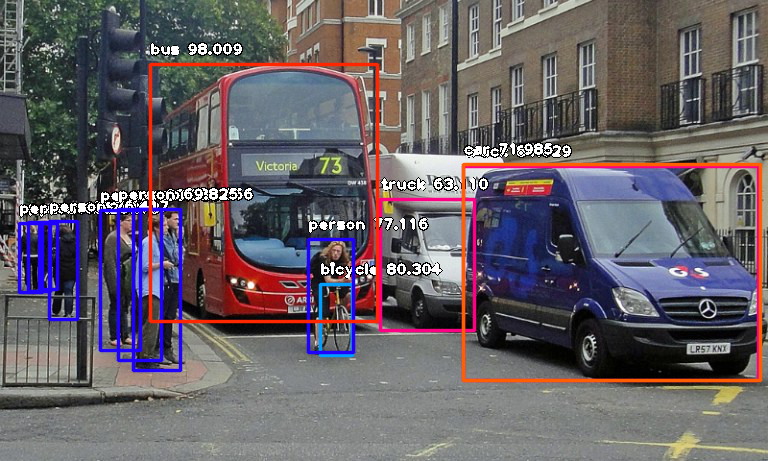
\includegraphics[width=11cm]{Obrazy/rozpoznawanieObiektow}
        \caption{Przykład rozpoznawania obiektów na zdjęciu ulicy. \cite{rozpoznawanieObiektow}}
        \label{fig.rozpoznawanieObiektow}
    \end{figure}

    Można znaleźć wiele witryn internetowych, które udostępniają interfejsy programistyczne umożliwiające zaimplementowanie
    rozpoznawania wieku z obrazu.
    Istnieją algorytmy przetwarzania obrazu, które oprócz wieku wyznaczają z pewnym prawdopodobieństwem płeć danej osoby.
    Oprócz płci mogą one także wyznaczyć mine oraz czy dana osoba nosi okulary.

    Z weryfikacją wieku danej osoby można się spotkać przed wejściem do niektórych miejsc, tj.
    klub nocny.
    Większość osób
    musi okazać ważny dowód osobisty,
    co generuje duże kolejki do wejścia.
    Aplikacje analizujące wiek na podstawie obrazu twarzy z kamery przed wejściem
    do takich miejsc znacząco usprawniłyby weryfikację wieku.
    Rozpoznawanie wieku może być wykorzystywane przy analizie średniego wieku ludzi w jakimś miejscu np.
    podczas demonstracji.

    Wiele gier posiada treści nieodpowiednie dla młodszych użytkowników.
    Możliwe jest stosowanie technologii wykrywania
    wieku użytkownika przed udostępnieniem mu treści, która wymaga odpowiedniego wieku.

    Można znaleźć o wiele więcej potencjalnych zastosowań przetwarzania obrazu oraz rozpoznawania wieku na podstawie
    tekstury (obrazu) twarzy.
    Z biegiem lat z pewnością będzie można zauważyć dalszy rozwój tej dziedziny, która
    opiera się w głównej mierze na sztucznej inteligencji \cite{computerVision}.
    %275 wyrazow

    %    \section{Cel i zakres pracy}
    %    Celem pracy magisterskiej jest stworzenie prostego programu do rozpoznawania wieku na podstawie tekstury twarzy.
    %
    %    Zakres pracy obejmuje:
    %    \begin{itemize}
    %        \item Wybór bazowej metody wyznaczania wieku
    %        \item Stworzenie kilku modyfikacji bazowej metody
    %        \item Opis algorytmów każdej z metod wyznaczania wieku
    %        \item Porównanie wszystkich metod i wybór najlepszej
    %    \end{itemize}
    %
    %    \chapter{Przegląd metod wyznaczania wieku}
    %    \section{Metoda a}
    %    \section{Metoda b}
    %    \section{Metoda wrinkle feature}

    \chapter{Metoda bazowa - wrinkle feature}
    %todo rozne metody
    Istnieje wiele metod wyznaczania wieku z obrazu twarzy.
    W literaturze spotkano rozwiązania, w których wyznaczany
    jest konkretny
    wiek osoby przez algorytm lub przedział wiekowy.
    Jedna z pierwszych metod szacowania wieku opierała się na wyznaczaniu proporcji twarzy, a następnie na detekcji i
    interpretacji zmarszczek.
    Była ona w stanie ze stu procentową poprawnością wyznaczyć czy dana osoba jest osobą
    dorosłą lub
    dzieckiem \cite{kwonLobo}.

    W kolejnych latach algorytmy i techniki szacowania wieku były udoskonalane.
    Badano wpływ starzenia się osób na
    wygląd skóry.
    Oprócz naturalnych zmian skóry pod wpływem starzenia się skóry należało uwzględnić także inne
    czynniki.
    Takimi czynnikami są min.
    płeć, poziom stresu, ekspozycja na działanie środowiska zewnętrznego.
    Powyższe metody zastosowano w pracy ,,Toward automatic simulation
    of aging effects on face images'' autorstwa A. Lanitis, Ch. J. Taylor oraz T. F. Cootes \cite{lanitisTaylor}.
    Należy dodać, że w powyższej pracy stosowano trenowanie zbioru zdjęć.
    Trenowanie polega na wykryciu relacji pewnych cech twarzy do wieku osób.

    W kolejnych latach pojawiło się podejście porównywania cech twarzy tej samej osoby w różnym wieku.
    Różnice w powyższych cechach posłużyły do zbudowania statystyki zmian cech twarzy wraz ze starzeniem się.
    Powyższe podejście zostało zaprezentowane w pracy ,,Face verification across age progression''
    autorstwa N. Ramanathan oraz R. Chellappa \cite{ramanthanChelappa}.

    Rozwinięciem tego pomysłu była praca ,,Automatic age estimation based
    on facial aging patterns'' autorstwa X. Geng, Z. Zhou i K. Smith-Miles \cite{gengZhou}.
    W tej pracy porównywano sekwencje wielu zdjęć twarzy jednej osoby.
    Zdjęcia przestawiały twarz w różnym wieku.
    Powyższe badania pozwoliły na zbudowanie wzorca starzenia się twarzy.

    Praca ,,A new algorithm for age recognition
    from facial images'' autorstwa M.M. Dehshibi oraz A. Bastanfard \cite{dehshibiBastard} przy szacowaniu wieku
    analizuje proporcje twarzy oraz ilość zmarszczek.

    Praca ,,Age Estimation from Face Images: Challenging
    Problem for Audience Measurement Systems'' autorstwa
    Vladimira Khryashcheva, Alexandra Ganina, Olgi Stepanovej oraz
    Antona Lebedeva podsumowała techniki szacowania wieku \cite{khryashchevGanin}.
    Z podsumowania wynikło, że najczęściej stosuje się do wyodrębniania cech z twarzy BIF,
    czyli biologically inspired features.
    Powyższa metoda została zaprezentowana w książce ,,Human Age Estimation Using Bio-inspired Features''
    autorstwa Guodong Guo i in.
    Mniej popularne metody analizujące cechy twarzy to filtry Gabora oraz LBP- local binary patterns.


    Metoda bazowa została opisana w artykule ,,Age Estimation from Face Image using Wrinkle Features''
    ~\cite{wrinkleFeatures}.
    Wykrywanie wieku dzieli się na kilka faz.
    Na początku należy wykryć twarz.
    Zastosowany algorytm wykrywania został
    opisany w sekcji \ref{sec:metodaWykrywaniaTwarzy}
    Następnie należy wyznaczyć strefy zmarszczkowe na twarzy.
    W artykule \cite{wrinkleFeatures} udowodniono,
    że istnieje kilka konkretnych stref, w których następuje znacząca zmiana ilości zmarszczek wraz z wiekiem.
    Powyższe strefy zostały wymienione w sekcji \ref{sec:wyznaczanieStref}.
    Sekcja \ref{sec:wykrywanieZmarszczek} przedstawia technikę wykrywania zmarszczek znajdujących się w strefach.
    Wykryte zmarszczki
    pozwalają na obliczenie wrinkle feature dla danej twarzy, zgodnie z opisem w sekcji \ref{sec:wyliczanieWrinkleFeature}.
    W tym miejscu kończy się faza wyznaczania wrinkle feature dla danej osoby (Rysunek \ref{fig.faza1Algorytmu}).
    Kolejna faza
    jest potrzebna do
    znalezienia relacji pomiędzy wrinkle feature a wiekiem.
    Do tego celu należy zastosować algorytm trenujący, który
    został opisany w sekcji \ref{sec:algorytmTrenowania}.
    Wynikiem algorytmu trenującego jest zbiór danych, który
    należy pogrupować, tak jak to opisano w sekcji \ref{sec:grupowanieDanych}.
    Ostatnią fazą algorytmu jest wykrywanie wieku
    na podstawie wyników działania FCM - sekcja \ref{sec:wyznaczanieWieku} (Rysunek \ref{fig.faza2Algorytmu}).

    \begin{figure}[h]
        \centering
        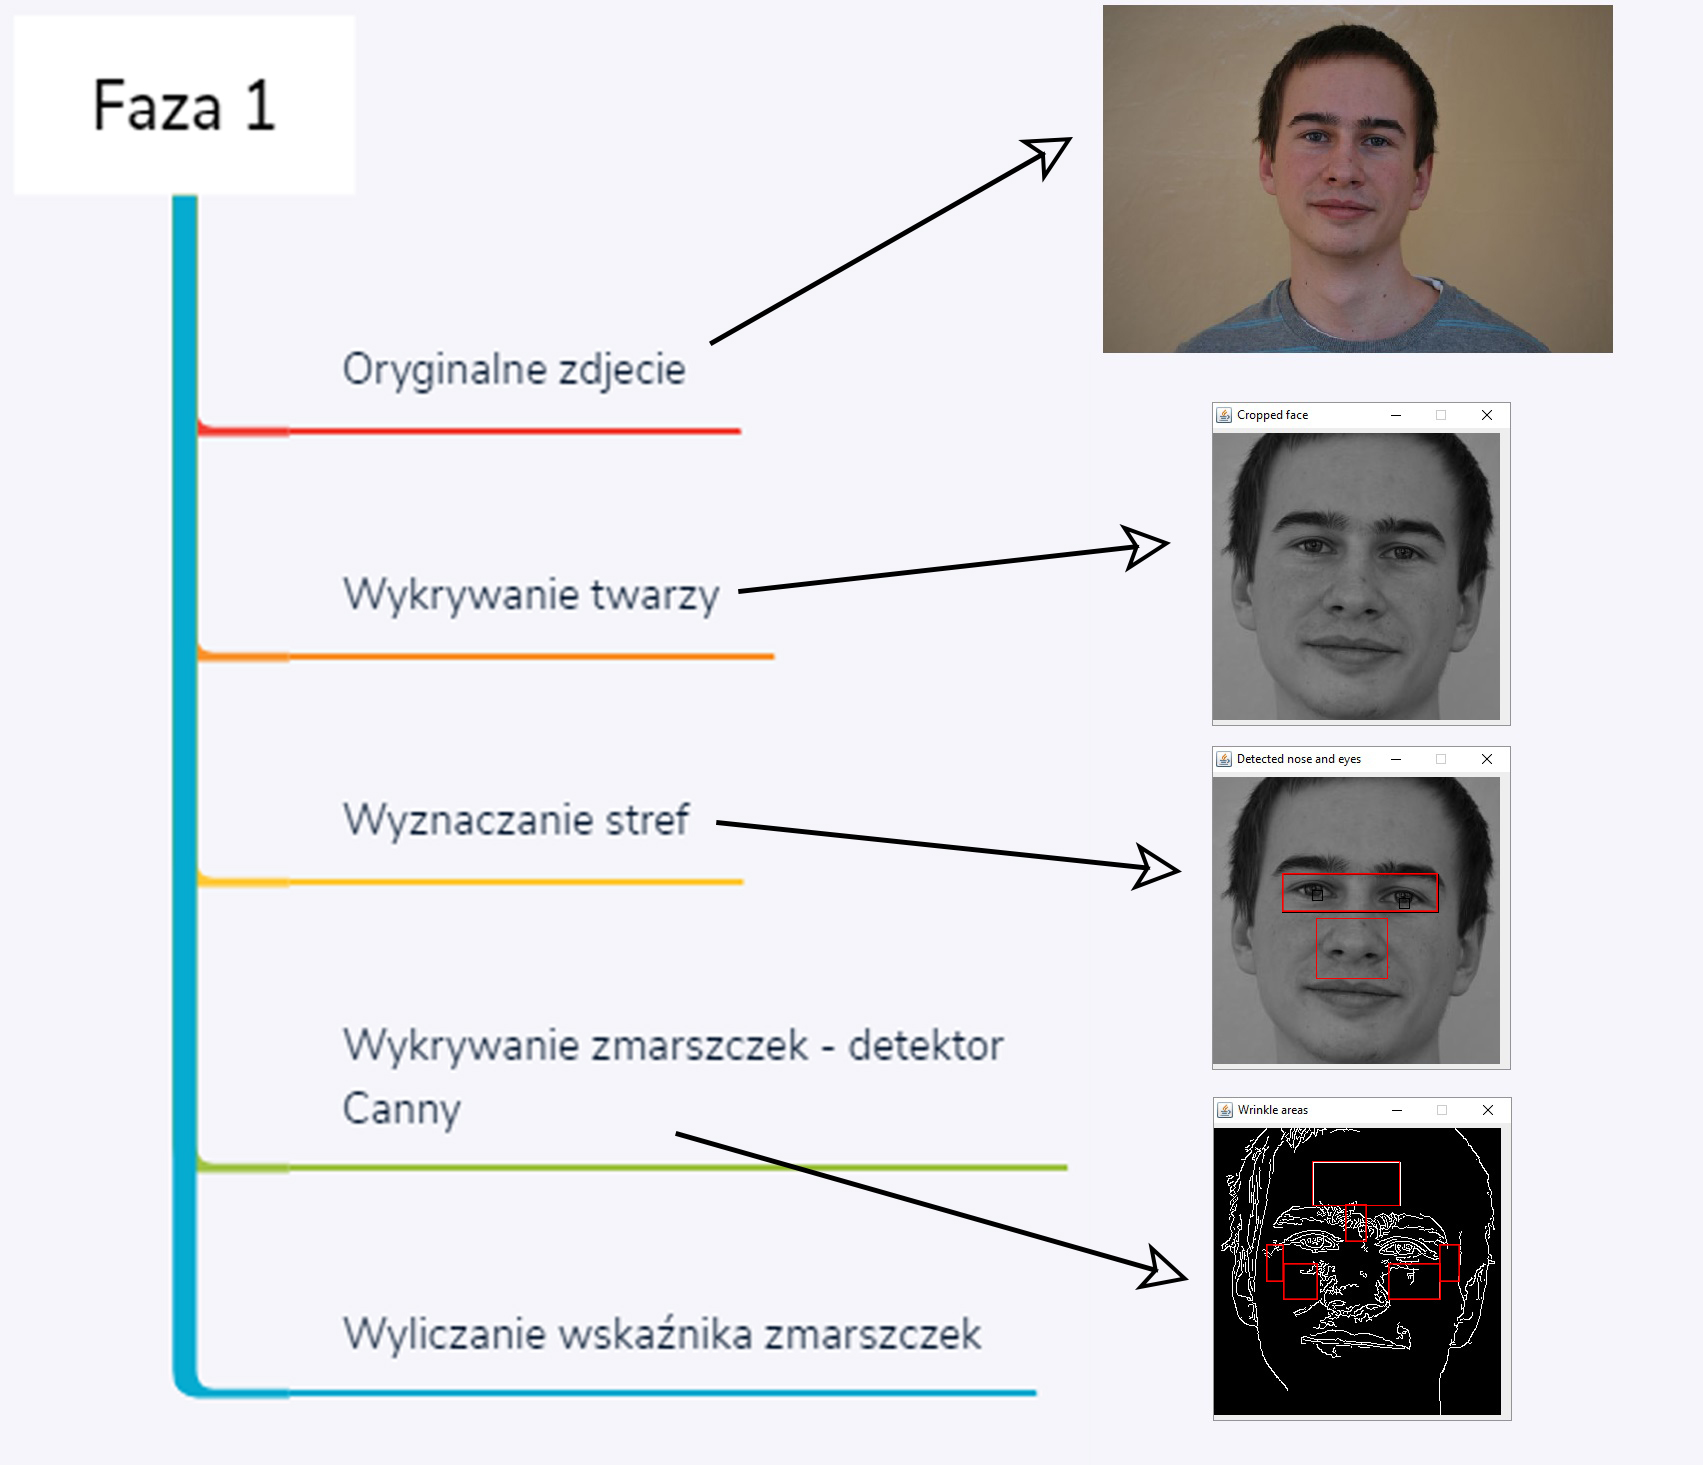
\includegraphics[width=8cm]{Obrazy/Faza1.jpg}
        \caption{Faza 1 algorytmu}
        \label{fig.faza1Algorytmu}
    \end{figure}

    \begin{figure}[h]
        \centering
        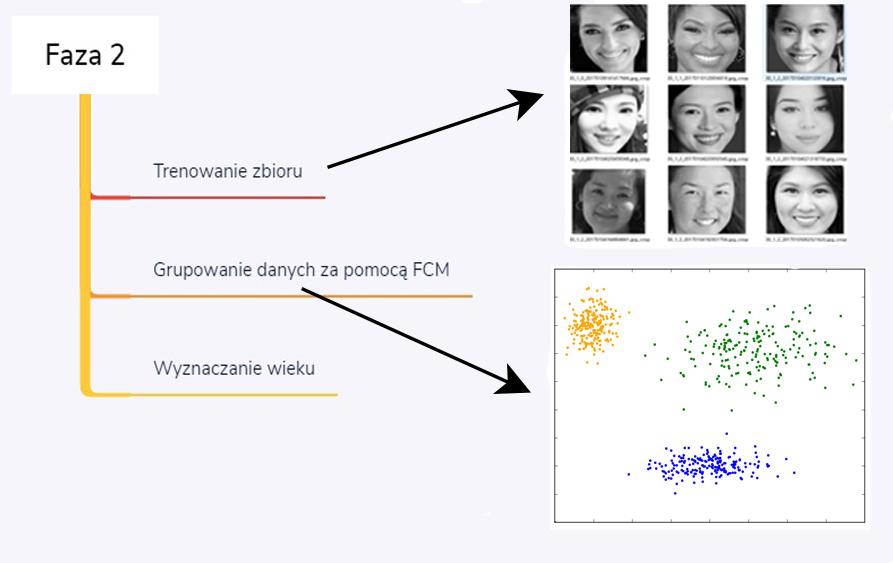
\includegraphics[width=8cm]{Obrazy/Faza2.jpg}
        \caption{Faza 2 algorytmu}
        \label{fig.faza2Algorytmu}
    \end{figure}

    \section{Metoda wykrywania twarzy}\label{sec:metodaWykrywaniaTwarzy}
    W literaturze można odnaleźć wiele metod wykrywania twarzy.
    Istnieje kilka podejść aby skutecznie wykrywać twarz na danym obrazie \cite{mehdiRizvi}:
    %       https://www.researchgate.net/publication/257338580_A_Review_on_Face_Detection_Methods
    %     Knowledge-based methods: These rule-based methods encode human knowledge
    %    of what constitutes a typical face. Usually, the rules capture the relationships
    %    between facial features. These methods are designed mainly for face localization.
    %     Feature invariant approaches: These algorithms aim to find structural features that
    %    exist even when the pose, viewpoint, or lighting conditions vary, and then use these
    %    to locate faces. These methods are designed mainly for face localization.
    %     Template matching methods: Several standard patterns of a face are stored to
    %    describe the face as a whole or the facial features separately. The correlations
    %    between an input image and the stored patterns are computed for detection. These
    %    methods have been used for both face localization and detection.
    %     Appearance-based methods: In contrast to template matching, the models (or
    %    templates) are learned from a set of training images which should capture the
    %    representative variability of facial appearance. These learned models are then used
    %    for detection. These methods are designed mainly for face detection.

    \begin{itemize}
        \item metoda oparta na nauce
        \item metoda niezmienności cech
        \item metoda dopasowania szablonu twarzy
        \item metoda bazująca na wyglądzie
    \end{itemize}
    Metoda oparta na nauce kieruje się wiedzą na temat wyglądu twarz.
    Dokładniej chodzi o charakterystyczne cechy,
    które pozwalają na wyodrębnienie obszaru twarzy na zdjęciu.
    Mowa tutaj o cechach takich jak kształt twarzy, kolor, miejsca o różnej jasności czy krawędzie tworzone np przez
    usta.

    Metoda niezmienności cech wyszukuje takie strukturalne cechy twarzy, które są widoczne w każdych warunkach
    oświetleniowych.
    Ponadto powyższe cechy są widoczne bez względu na punkt widzenia np.
    profil czy kąt nachylenia twarzy.

    Metoda dopasowania szablonu twarzy wykorzystuje kilka standardowych wzorów opisujących twarz.
    Na wejściu algorytmu obraz jest porównywany z powyższymi wzorami.
    Na wyjściu dostajemy informację w jakim stopniu obraz jest dopasowany do szablonu twarzy.

    Ideą metody bazującej na wyglądzie jest trenowanie dużego zbioru obrazów twarzy, tak aby wychwycić zmienność cech
    twarzy.
    Tak wytrenowany model jest później wykorzystywany do wykrywania twarzy.


    Ponadto w procesie ekstrakcji twarzy z obrazu istnieje wiele problemów  \cite{mehdiRizvi}.
    %       https://www.researchgate.net/publication/257338580_A_Review_on_Face_Detection_Methods
    %    Pose: The images of a face vary due to the relative camera-face pose (frontal, 45
    %    degree, profile, upside down), and some facial features such as an eye or the nose
    %    may become partially or wholly occluded.
    %     Presence or absence of structural components: Facial features such as beards,
    %    mustaches, and glasses may or may not be present and there is a great deal of
    %    variability among these components including shape, color, and size.
    %     Facial expression: The appearance of faces is directly affected by a person’s facial
    %    expression.
    %     Occlusion: Faces may be partially occluded by other objects. In an image with a
    %    group of people, some faces may partially occlude other faces.
    %     Image orientation: Face images directly vary for different rotations about the
    %    camera’s optical axis.
    %     Imaging conditions: When the image is formed, factors such as lighting (spectra,
    %    source distribution and intensity) and camera characteristics (sensor response,
    %    lenses) affect the appearance of a face.
    %    Każda z nich wyodrębnia z obrazu pewne cechy, które
    %    mogą wskazywać, że na danym obszarze obrazu znajduje się twarz.

    Jednym z nich jest nieodpowiednia poza.
    Wiąże się to z różnymi ustawieniami twarzy wobec aparatu fotograficznego lub kamery.
    Twarz może być nachylona, przechylona, odchylona.
    Inaczej mówiąc może mieć różne położenie w trzech wymiarach.
    Niektóre części twarzy lub cechy mogą zostać przysłonięte.
    Im mniej cech widocznych na twarzy tym mniej danych, które algorytm może wyodrębnić z twarzy.
    Im mniej danych posiada algorytm tym mniejsze prawdopodobieństwo prawidłowego wykrycia twarzy.

    Pewne twarze mogą zawierać lub nie pewne cechy tj. brody, blizny, okulary.
    Różnorodność tych cech także wpływa na efektywność wykrywania twarzy.

    Wyrazy mimiczne wpływają na zwiększenie ilości zmarszczeń na twarzy.
    Ponadto zmienia się kształt ust, pojawiają się ostre krawędzie wynikające z pracy mięśni twarzowych.
    Widoczne mogą być różne pofałdowania skóry.

    Zdarza się, że część twarzy zostaje przysłonięta przez jakiś inny obiekt.
    Na zdjęciu na którym jest wiele osób część twarzy może być przysłonięta przez inną twarz.
    Przysłonięcie przez inny obiekt wiąże się z utratą informacji o części twarzy co zmniejsza prawdopodobieństwo
    prawidłowego wykrycia twarzy.

    Istotnym elementem jest także oświetlenie twarzy.
    Gdy twarz oświetlona jest tzw. twardym światłem występują na
    niej tzw. ostre cienie i światła \ref{fig.oswietlenieTwarzy}.
    \begin{figure}
        \centering
        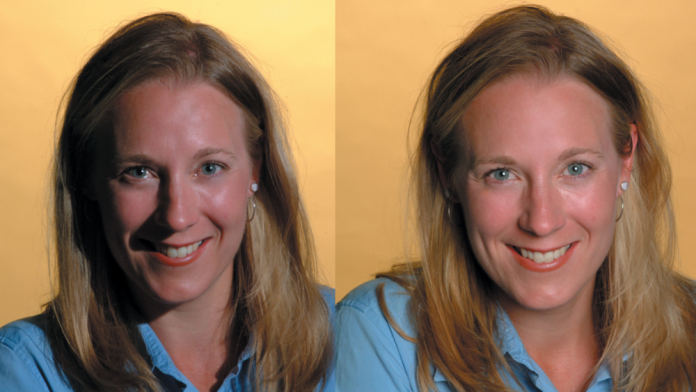
\includegraphics[width=12cm]{Obrazy/oswietlenieTwarzy.jpg}
        \caption{Przykład twarzy oświetlonej twardym (twarz po lewej) oraz miękkim światłem. \cite{oswietlenieTwarzy}}
        \label{fig.oswietlenieTwarzy}
    \end{figure}
    W tym przypadku występuje większe ryzyko utraty szczegółów oświetlanej twarzy.
    Gdy twarz jest skierowana na wprost słońca z dużym
    prawdopodobieństwem można powiedzieć, że zostanie oświetlona twardym światłem.
    Miękkie światło jest generowane na przykład przez zachmurzone niebo.
    Istotne jest także źródło światła.
    Źródło może być punktowe lub rozproszone.
    Przy punktowym źródle światła twarz będzie
    posiadać jednolity cień, którego intensywność będzie zależała od "twardości" światła.
    Przy świetle rozproszonym intensywność cieni zostanie zmniejszona.

    Na Rys \ref{fig.technikiWykrywaniaTwarzy} przedstawione są różne techniki wykrywania twarzy.
    \begin{figure}
        \centering
        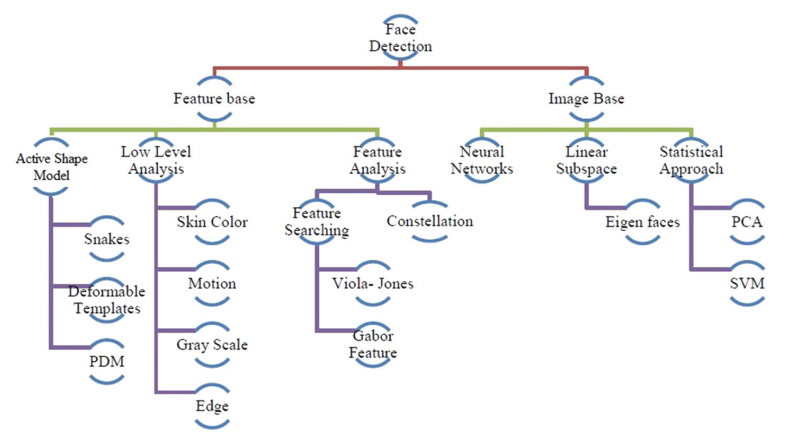
\includegraphics[width=15cm]{Obrazy/technikiWykrywaniaTwarzy.jpg}
        \caption{Różne techniki wykrywania twarzy. \cite{faceDetectionTechniques}}
        \label{fig.technikiWykrywaniaTwarzy}
    \end{figure}
    %    https://sci-hub.tw/10.1007/s10462-018-9650-2

    %    Wyodrębnianie lub ekstrakcja cech polega na przekształceniu obrazu do zbioru zmiennych, które
    %    zostaną później użyte w wykrywaniu obiektu lub obiektów na obrazie.

    Jak widać metod wykrywania twarzy jest sporo.
    Omówienie każdej z nich zajęłoby dużo czasu.
    Poniżej zostaną przytoczone dwie metody wykrywania twarzy.
    Dodatkowo zostanie omówiona metoda, która posłużyła do wykrywania twarzy w niniejszej pracy.

    %https://sci-hub.tw/10.1016/S0031-3203(00)00134-5
    W pracy ,,An efficient algorithm for human face detection and facial
    feature extraction under different conditions'' (\cite{wongLamSiu})
    przedstawiono opisaną w skrócie poniżej technikę wykrywania twarzy.
    W pierwszym etapie procesu obszary, gdzie może znajdować się ludzkie oko,
    są wykrywane przez przeprowadzenie testów na zacienionych rejonach obrazu.
    Pary takich obszarów wyodrębnia się na podstawie algorytmu genetycznego,
    aby następnie wyznaczyć możliwy obszar twarzy.
    Dla każdego obszaru mierzy się wartość dopasowania na podstawie jego projekcji na wektory własne,
    tzw. eigenfaces.
    Aby wiarygodność wykrywania była wyższa,
    każdy możliwy obszar twarzy normalizuje się pod kątem oświetlenia.
    Proces ten powtarza się pewną ilość razy,
    a następnie do dalszej weryfikacji są wybierane możliwe obszary twarzy o wysokiej wartości dopasowania.
    Na tym etapie mierzy się symetrię twarzy oraz sprawdza się,
    czy na każdym wybranym obszarze istnieją rysy twarzy.
    Rysy określa się przez ewaluację rzeźby topograficznej - wystających i wklęsłych elementów
    różnych regionów obszaru twarzy, poddanego uprzednio normalizacji.
    Algorytm jest w stanie wykryć także obszar twarzy, gdy głowa jest przechylona

    %todo Druga metoda wykrywania twarzy z https://www.researchgate.net/publication/334770252_An_Accurate_System_for_Face_Detection_and_Recognition
    %todo https://sci-hub.tw/10.1007/s10462-018-9650-2
    W roku 1997 w pracy pt. ,,Vision for man-machine interaction'' opisano metodę wykrywania twarzy bazującą na
    wykrywaniu cechy jaką jest kolor skóry \cite{clowleyCoutaz}.
    Kolor skóry jest najbardziej widoczną cechą twarzy zarówno dla człowieka jak i dla maszyny.
    Ponadto kolor jest przetwarzany znacznie szybciej od innych cech.
    Przy dobrych warunkach oświetleniowych ustawienie twarzy nie ma wpływu na skuteczność wykrywalności twarzy
    opisywaną metodą.
    Każda metoda wykrywania twarzy posiada wady.
    Jedną z tych wad jest problem wykrywalności twarzy przy nierównomiernym oświetleniu.
    Problem pojawia się także, gdy na obrazie widoczny jest obszar skóry z poza twarzy np. z rąk.
    Warto zaznaczyć, że kolor twarzy na obrazie jest zależny od względnego kierunku oświetlenia.
    Obszar twarzy w omawianym algorytmie jest wykrywany poprzez normalizacje histogramu kolorów.
    Normalizacja jest potrzebna do redukcji wpływu luminancji na kolor.

    %todo trzecia metoda  - wstep do Haar Cascade https://drive.google.com/file/d/1nJ9S3HtuuFY6O1FLdIjRWSzWUFwZ_fuJ/view?usp=sharing
    Algorytm Haar Cascade jest najpopularniejszym algorytmem do wykrywania twarzy w bibliotece OpenCV. Właśnie ta
    biblioteka była jednym z niezbędnym elementów programu przy wykrywaniu wieku z tekstury twarzy.
    W związku z powyższym w wykrywaniu twarzy zastosowano algorytm Haar Cascade.
    Omawiany algorytm został zaprezentowany w książce ,,Rapid Object Detection using a Boosted Cascade of Simple
    Features'' w 2001 i składa się z trzech faz \cite{violaJones}.
    W pierwszej obraz wejściowy przekształcany jest na obraz scałkowany.
    Następnie wykorzystywany jest algorytm do boostingu, który zmniejsza ilość klasyfikatorów tylko do tych
    najbardziej istotnych.
    W ostatniej fazie klasyfikatory łączone są w kaskady w celu przyspieszenia procesu wykrywania twarzy.
    Znaczna większość metod wykrywania obiektów na obrazie (w tym twarzy) wymaga wstępnego przekształcenia obrazu do
    skali szarości.

    %    https://towardsdatascience.com/face-recognition-with-opencv-haar-cascade-a289b6ff042a
    %    przez kogo został zaproponowany...
    %    byc moze cos o funkcji kaskadowej
    %    o tym ze OpenCv zawiera wytrenowane algorytmy Haar Cascade ktore wykrywaja ryj, oczy, usta itp
    %    wkleic obrazek z rodzajami filtrow
    %    jak dziala ten filtr
    %    przyklad na gebie emmy watson moze...
    %cosik tam jeszcze

    %    opisac jak dokladnie zaimplementowano to u nas
    %    przejscie na skale szarosci podczas wykrywania... czym ona jest?...
    \subsection{Konwersja do skali szarości oraz przestrzenie barw}\label{subsec:konwersja-do-skali-szarości-oraz-przestrzenie-barw}
    %todo https://sci-hub.tw/10.1007/s10462-018-9650-2
    Każdy piksel w trybie kolorowym ma określoną reprezentację barwy z określonego modelu.
    Najczęściej są to 3 lub 4 wartości \cite{przestrzenieKolorow}.
    Pierwszą przestrzenią barw była CIEXYZ. Została ona stworzona w 1931 przez
    Międzynarodowa Komisja ds. Oświetlenia (International Commission on Illumination).
    Przestrzeń barw CIEXYZ została specjalnie stworzona, by odtworzyć sposób postrzegania barw przez ludzkie oko.
    Barwa jest opisywana w trzech współrzędnych trójchromatycznych X,Y,Z.
    Powyższe współrzędne są zależne od składowych - sprawności wizualnych czopków.
    Czopki to światłoczułe receptory siatkówki ludzkiego oka \cite{przestrzenieKolorow}.
    Współrzędne X,Y,Z wyliczane są na podstawie trzech podstawowych barw R (czerwonej),
    G (zielonej) i B (niebieskiej).
    Współrzędne XYZ są często reprezentowane przez luminancję Y oraz współrzędne x, y chromatyczności.
    Wyliczanie współrzędnych x, y przedstawiono na wzorach \ref{wzor.chromX} oraz \ref{wzor.chromY}.
    \large
    \begin{equation}
        x = \frac{X}{X+Y+Z}
        \label{wzor.chromX}
    \end{equation}
    \normalsize

    \large
    \begin{equation}
        y = \frac{Y}{X+Y+Z}
        \label{wzor.chromY}
    \end{equation}
    \normalsize

    Na rysunku \ref{fig.CIEXYZ} przedstawiono diagram chromatyczności reprezentujący przestrzeń barw CIEXYZ.

    \begin{figure}
        \centering
        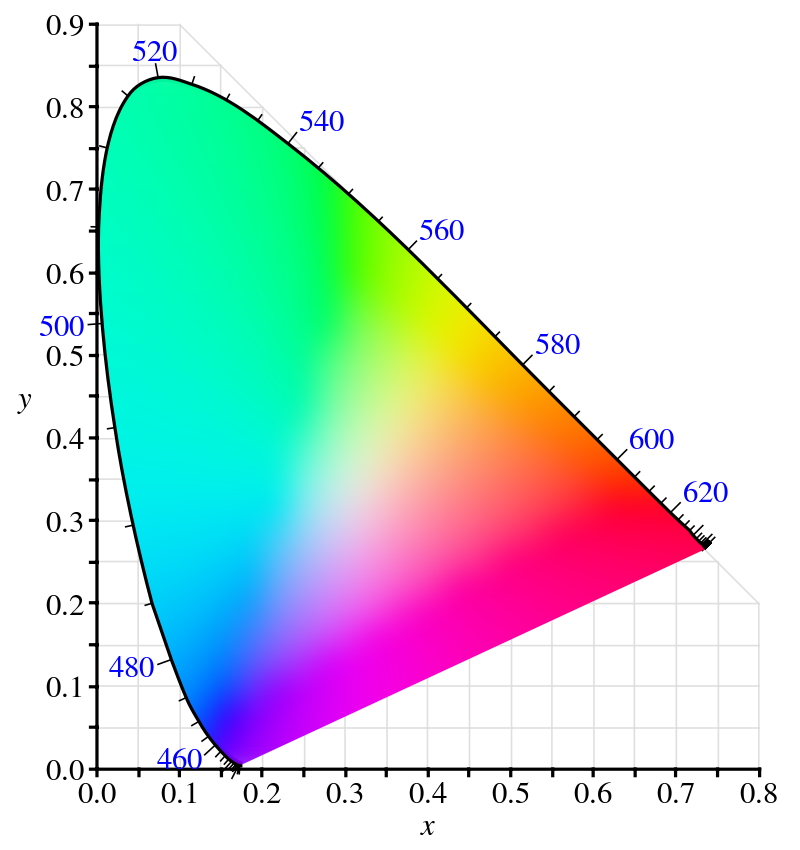
\includegraphics[width=6cm]{Obrazy/CIEXYZ.jpg}
        \caption{Przykład rozpoznawania obiektów na zdjęciu ulicy. \cite{diagramCIEXYZ}}
        \label{fig.CIEXYZ}
    \end{figure}

    Kolory mogą byc także odwzorowane przez przestrzeń barw CMYK.
    Skrót CMYK oznacza odpowiednio:
    \begin{itemize}
        \item Cyan - odcień niebieskiego
        \item Magenta - kolor karmazynowy
        \item Yellow - kolor żółty
        \item K - key colour - kolor czarny
    \end{itemize}
    Barwa wynikowa powstaje poprzez mieszanie trzech kolorów - niebieskiego, karmazynowego oraz żółtego.
    Mieszanie zachodzi według zasady syntezy subtraktywnej \cite{przestrzenieKolorow}.
    Synteza subtraktywna polega na mieszaniu kolorów przez odejmowanie promieniowań widzialnych różnych długości.
    Przykładem syntezy subtraktywnej jest np. mieszanie farb o różnych kolorach.

    Najczęściej barwy są reprezentowane przez przestrzeń barw RGB \cite{przestrzenieKolorow}.
    Przestrzeń kolorów RGB składa się z trzech kanałów
    \cite{kolory}:

    \begin{itemize}
        \item R - czerwonego (z angielskiego Red)
        \item G - zielonego (z angielskiego Green)
        \item B - niebieskiego (z angielskiego Blue)
    \end{itemize}
    Barwy mieszane są poprzez syntezę addytywną .
    W przeciwieństwie do syntezy subtraktywnej barwa wynikowa powstaje poprzez sumowanie wiązek światła widzialnego o
    różnych długościach \cite{przestrzenieKolorow}.
    Każdy piksel opisany za pomocą przestrzenie barw RGB ma trzy 8-bitowe wartości reprezentujący każdy kanał.
    Spotykane
    są 12- lub 16-bitowe reprezentacje kanałów, jednak 8-bitowa jest najpopularniejsza.
    Dla 8-bitowych kanałów
    wartość ,,0''
    danego kanału oznacza brak jasności, natomiast ,,255'' maksymalną jasność.
    Poprzez mieszanie jasności tych trzech kanałów
    można uzyskać szerokie spektrum barw (Rysunek \ref{fig.mieszanieKolorow}).

    \begin{figure}
        \centering
        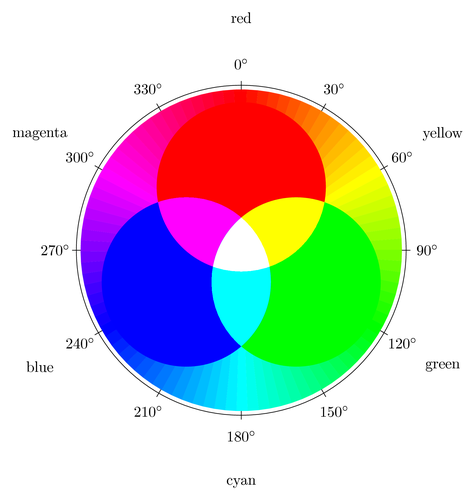
\includegraphics[width=7cm]{Obrazy/mieszanieKolorow.jpg}
        \caption{Mieszanie kanałów RGB. \cite{colorMixing}}
        \label{fig.mieszanieKolorow}
    \end{figure}

    Przykładowo kolor o reprezentacji R=153 G=217 B=234 przedstawiono na Rysunku \ref{fig.mieszanieKolorowBlekitny}

    \begin{figure}
        \centering
        
\includegraphics[width=2cm]{Obrazy/blekitny.jpg}
        \caption{Kolor R=153 G=217 B=234.}
        \label{fig.mieszanieKolorowBlekitny}
    \end{figure}

    Kolor (Rysunek \ref{fig.mieszanieKolorowBlekitny}) może być też reprezentowany w kodzie szesnastkowym \#99D9EA.
    Każda
    wartość heksadecymalna odpowiada kolejno kanałowi R, G, B.

    Obraz może też być przedstawiony stosując odcienie jednej barwy.
    Taka obraz nazywa się obrazem monochromatycznym.
    Najczęściej stosowaną barwą w takich obrazach jest szarość \cite{przestrzenieKolorow}.

    Istnieją 3 metody konwersji obrazu z przestrzeni RGB na monochromatyczny \cite{colorMixing}.
    \begin{itemize}
        \item największej jasności
        \item średnia
        \item luminancji
    \end{itemize}
    Metoda największej jasności konwertuje na skalę szarości wg wzoru \ref{wzor.najwiekszaJasnosc}.

    \large
    \begin{equation}
        \frac{(max(R, G, B) + min(R, G, B))}{2}
        \label{wzor.najwiekszaJasnosc}
    \end{equation}
    \normalsize
    Metoda średnia bazuje na wzorze \ref{wzor.metodaSrednia}, natomiast metodę luminancji ilustruje wzór
    \ref{wzor.metodaLuminancji}.

    \large
    \begin{equation}
        \frac{(R + G + B)}{3}
        \label{wzor.metodaSrednia}
    \end{equation}
    \normalsize

    \large
    \begin{equation}
        0.21 R + 0.72 G + 0.07 B
        \label{wzor.metodaLuminancji}
    \end{equation}
    \normalsize

    W niniejszej pracy zastosowano konwersję za pomocą metody średniej.
    \subsection{Algorytm Haar Cascade}\label{subsec:algorytm-haar-cascade}

    Haar Cascade jest algorytmem z dziedziny uczenia maszynowego służącym do wykrywania obiektów w wizji komputerowej.
    Został stworzony przez Paula Viola oraz Michaela Jonesa \cite{violaJones}.
    Opiera się na zbudowaniu kaskadowej funkcji za pomocą trenowania wielu zdjęć.
    Zdjęcia są dzielone na
    dwie kategorie - pozytywne oraz negatywne.
    Na zdjęciach klasyfikowanych jako pozytywne istnieje obiekt, który ma zostać wykryty, natomiast
    na zdjęciach negatywnych nie ma tego obiektu.

    Ekstrakcja cech w algorytmie Violi i Jonesa jest realizowana przez filtry Haara.
    Są to prostokątne okienka
    nakładane na obraz, które analizują jasność pikseli (Rysunek \ref{fig.haarRectangles}).
    \begin{figure}
        \centering
        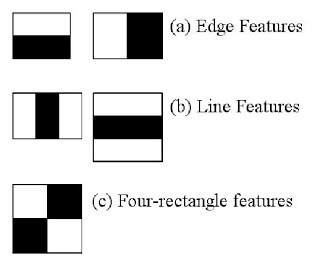
\includegraphics[width=7cm]{Obrazy/Haar_filter_rectangles.jpg}
        \caption{Filtr Haara a) krawędziowy b) liniowy c) szachownica \cite{haar}}
        \label{fig.haarRectangles}
    \end{figure}

    Przed zastosowaniem filtru Haara obraz musi zostać przekształcony do skali szarości
    W niniejszej pracy należało przekształcić każdy obraz z trybu kolorowego na monochromatyczny co opisano w sekcji
    \ref{subsec:konwersja-do-skali-szarości-oraz-przestrzenie-barw}.

    Każde okienko zawiera białe oraz czarne prostokąty.
    Wyznaczana jest suma jasności pikseli w obu rodzajach prostokątów, a
    następnie dla każdego okna obliczana jest różnica pomiędzy białymi a czarnymi.
    Opisywany algorytm ma zastosowanie w wykrywaniu krawędzi.
    Na granicy krawędzi istnieje różnica w jasności pikseli
    (Rysunek \ref{fig.haarEmmaWatson}).

    \begin{figure}
        \centering
        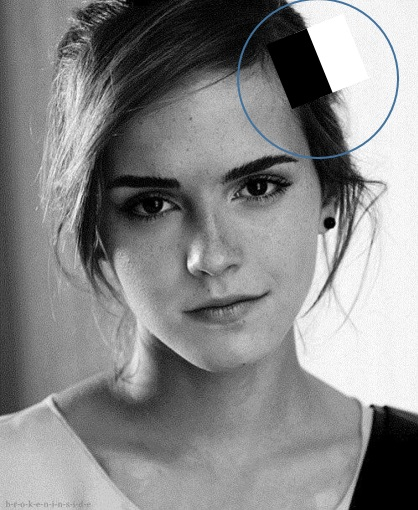
\includegraphics[width=6cm]{Obrazy/haarEmmaWatson.jpg}
        \caption{Filtr Haara nałożony na krawędź twarzy \cite{haar}}
        \label{fig.haarEmmaWatson}
    \end{figure}

    Podczas treningu klasyfikatora
    a każdego obrazu otrzymujemy dużą ilość danych.
    W celu poprawy efektywności sumowania pikseli w filtrze Haara stosowane są
    rozwiązanie zwane w języku angielskim Summed-area table \cite{violaJonesRealTimeOb}.Summed-area table jest również
    nazywana w literaturze Integral Image, czyli obrazem scałkowanym.
    Ideą obrazu scałkowanego jest,
    aby każdy obraz
    został
    przekształcony w
    tabelę, w której każdy element x,y tej tabeli odpowiada sumie jasności wszystkich pikseli według wzoru \ref{wzor
    .summedAreaTable}.

    \large
    \begin{equation}
        I(x,y) = \sum_{{x}'\leq x \cap {y}'\leq y}^{} i({x}',{y}')
        \label{wzor.summedAreaTable}
    \end{equation}
    \normalsize
    gdzie I(x,y) jest wartością na pozycji x,y w tabeli(tabela obrazu scałkowanego), i(x,y) - jasność piksela o
    współrzędnych x,y na obrazie.

    Na Rysunku \ref{fig.przedCalkowaniem} przedstawiona jest tabela prezentująca jasność pikseli przed
    zastosowaniem całkowania obrazu.
    \begin{figure}
        \centering
        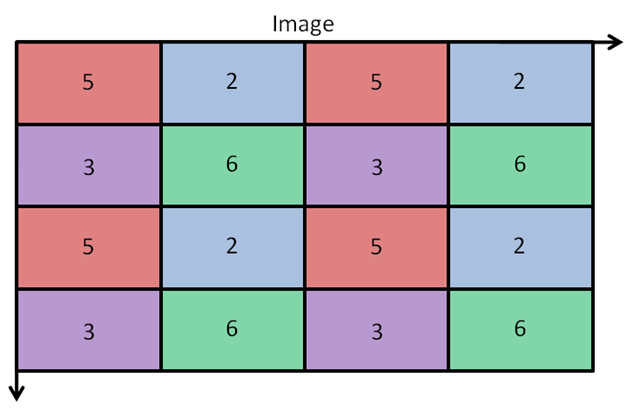
\includegraphics[width=6cm]{Obrazy/przedCalkowaniem.jpg}
        \caption{Tabela jasności poszczególnych pikseli przed zastosowaniem całkowania \cite{integralImages}}
        \label{fig.przedCalkowaniem}
    \end{figure}

    Po całkowaniu otrzymujemy tabelę podobną do przedstawionej na Rysunku \ref{fig.poCalkowaniu}.
    \begin{figure}
        \centering
        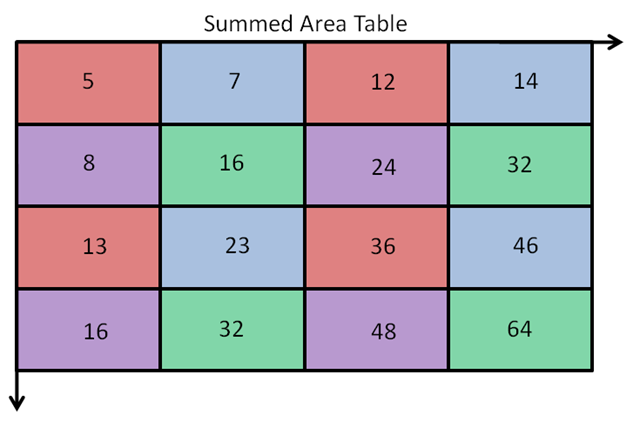
\includegraphics[width=6cm]{Obrazy/poCalkowaniu.jpg}
        \caption{Filtr Haara nałożony na krawędź twarzy \cite{integralImages}}
        \label{fig.poCalkowaniu}
    \end{figure}

    Sumowanie przykładowego okna (Rysunek \ref{fig.sumowanieOkna}) wymaga 4 operacji (Wzór \ref{wzor.windowsSum}).
    \begin{figure}
        \centering
        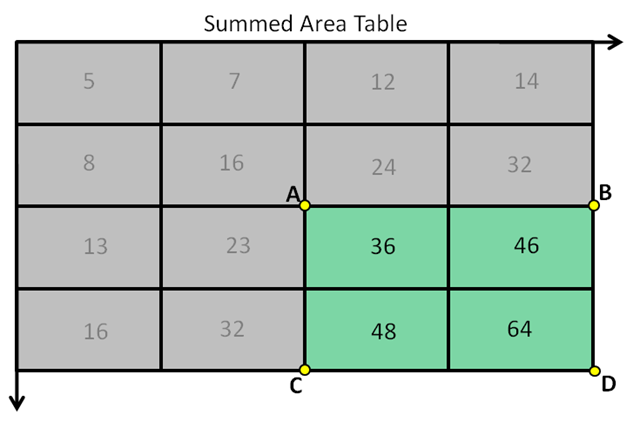
\includegraphics[width=6cm]{Obrazy/sumowanieOkna.jpg}
        \caption{Sumowanie okna \cite{integralImages}}
        \label{fig.sumowanieOkna}
    \end{figure}


    \large
    \begin{equation}
        \sum_{x_0\leq x \leq x_1\cap {y}\leq y \leq y_1}^{} i(x,y) = I(D) + I(A) - I(B) - I(C)
        \label{wzor.windowsSum}
    \end{equation}
    \normalsize
    gdzie lewa część równania oznacza sumę jasności pikseli
    zaznaczonego okna tj.
    na Rysunku \ref{fig.sumowanieOkna}, I(A) - wartość scałkowanego obrazu przy punkcie A
    (analogicznie I(B), I(C), I(D)) - (Rysunek \ref{fig.sumowanieOkna}).

    Zakładając większy rozmiar okna np. \begin{math}
                                            9x9
    \end{math} sumowanie okna zwykłym sposobem
    wymagałoby \begin{math}
                   9x9=81
    \end{math} operacji.
    Natomiast przy użyciu obrazu scałkowanego liczba operacji jest
    stała i wynosi dokładnie 4 \cite{violaJones}.

    Liczba cech wykrywanych w zdjęciu za
    pomocą filtru Haara wynosi zwykle powyżej stu tysięcy \cite{violaJones}.
    Wiele z nich nie ma
    większego znaczenia w procesie wykrywania twarzy.
    Natomiast przy tak dużej ilości cech na obrazie potrzebna jest dodatkowa
    technika, która przyspieszy detekcję twarzy.
    Taką właśnie techniką jest AdaBoost.
    Została ona opracowana
    przez Yoava Freunda oraz Roberta Schapire'a. \cite{dataMiningInferencePrediction}.

    Główną koncepcją tego algorytmu jest wyodrębnienie najlepszych cech z obrazu, które następnie są używane do
    wytworzenia silnych klasyfikatorów.
    Silny klasyfikator powstaje jako liniowa kombinacja słabych
    klasyfikatorów ważonych.
    Z kolei słabe klasyfikatory są reprezentowane przez dane, które nie miały istotnego wpływu przy wykrywaniu pożądanego
    obiektu \cite{dataMiningInferencePrediction}.

    W ostatniej fazie stosowany jest algorytm kaskady klasyfikatorów.
    Klasyfikatory są podzielone na grupy i
    połączone ze sobą kaskadowo.
    W algorytmie każda grupa może podjąć dwie decyzje - przekazanie danych z klasyfikatorów
    do kolejnej grupy lub ich odrzucenie.
    Ma to na celu odrzucenie wielu negatywnych danych z klasyfikatorów \cite{cascade}.

    Biblioteka OpenCV zawiera wytrenowane klasyfikatory, które zostały użyte w tej pracy magisterskiej.
    Wykorzystano
    je do wykrycia twarzy, ust oraz oczu.
    Klasyfikatory mają postać plików xml, które można znaleźć na oryginalnym
    repozytorium projektu OpenCv.

    %1600 wyrazow
    \section{Wyznaczanie stref}\label{sec:wyznaczanieStref}

    \section{Wykrywanie zmarszczek - detektor Canny}\label{sec:wykrywanieZmarszczek}

    \section{Wyliczanie wrinkle feature}\label{sec:wyliczanieWrinkleFeature}

    \section{Algorytm trenowania}\label{sec:algorytmTrenowania}

    \section{Grupowanie danych - FCM}\label{sec:grupowanieDanych}

    \subsection{Wstęp do grupowania danych}
    \subsection{Metoda FCM}

    \section{Wyznaczanie wieku}\label{sec:wyznaczanieWieku}


    %Tutaj powinno byc 5000 slow

    \chapter{Modyfikacje metody bazowej}

    \section{Odjęcie wybranej strefy}

    \subsection{Zmiana algorytmu względem metody bazowej}

    \section{Zastosowanie metody HOG}
    \subsection{Opis algorytmu HOG}
    \subsection{Zastosowanie w projekcie}

    \section{Metoda HOG oraz grupowanie KNN}
    \subsection{Grupowanie KNN}
    \subsection{Zastosowanie w projekcie}
    %Tutaj powinno byc okolo 7000
    \chapter{Badania}

    %opisywac nie tylko wyniki ale tez posrednio co tam lecialo, statystyki, szybkosc dzialania (sredni czas
    %    przetwarzania), zajetosc pamieci
    \chapter{Podsumowanie}



    %%%%%%%%%%%%%%%%%%%%%%%%%%%%%%%%%%%%%%%%%%
    \backmatter
    \pagenumbering{Roman}
    \stepcounter{stronyPozaNumeracja}
    \setcounter{page}{\value{stronyPozaNumeracja}}

    \pagestyle{tylkoNumeryStron}

    %%%%%%%%%%% bibliografia %%%%%%%%%%%%
    \bibliographystyle{plplain}
    \bibliography{bibliografia}

    %%%%%%%%%  DODATKI %%%%%%%%%%%%%%%%%%%

    \begin{appendices}


        \chapter*{Dokumentacja techniczna}

        \chapter*{Spis skrótów i symboli}

        \begin{itemize}
            \item[DNA] kwas deoksyrybonukleinowy (ang. \ang{deoxyribonucleic acid})
            \item[MVC] model -- widok -- kontroler (ang. \ang{model--view--controller})
            \item[$N$] liczebność zbioru danych
            \item[$\mu$] stopnień przynależności do zbioru
            \item[$\mathbb{E}$] zbiór krawędzi grafu
            \item[$\mathcal{L}$] transformata Laplace'a
        \end{itemize}




        \chapter*{Zawartość dołączonej płyty}

        Do pracy dołączona jest płyta CD z~następującą zawartością:
        \begin{itemize}
            \item praca w~formacie \texttt{pdf},
            \item źródła programu,
            \item zbiory danych użyte w~eksperymentach.
        \end{itemize}

        \listoffigures
        \listoftables

    \end{appendices}


\end{document}


%% Finis coronat opus.